% !TeX root = ../script.tex

\section{Krylov-Raum-Methoden für EW-Probleme}
Wir verfolgen die gleiche Idee, wie auch schon bei linearen Gleichungssystemen, d.h. die ursprünglich hochdimensionalen
Probleme, werden durch geeignete Unterräume (Krylov-Räume) in kleinere Probleme umgewandelt. \\
Wir erhalten dabei ein iteratives Vorgehen, zu betrachtende Beispiele sind die Arnoldi-Methode und die 
Lanczos-Methode.

Wir betrachten also die Eigenwertgleichung $Az=\lambda z$ mit $A\in\C^{n\times n}$ 
(ab jetzt erlauben wir auch komplexe Matrizen), wobei $A$ eine sehr große
Matrix ist, typischerweise $n\geq 10^4$.

\subsection{Galerkin-Approximation}
Eigenwertprobleme können äquivalent in Variationsform (schwache Formulierung) geschrieben werden, diese besagt: \\
$z\in\C^n$ ist genau dann ein Eigenvektor von $A$ zum Eigenwert $\lambda\in\C$, wenn
%
\begin{align*}
  \langle Az,y\rangle_2 
  = \lambda\langle z,y\rangle_2 \quad\forall\,y\in\C^n 
  \tag{1}\label{eq:galerkinEQ1}
\end{align*}
%
Diese Äquivalenz gilt, da aus $\langle r, y\rangle_2 = 0$ für alle $y\in\C^{n}$ folgt, dass $r=0$ sein muss, 
in unserem Fall ist $r=Az-\lambda z$ das Residuum des Eigenwertproblems.

Sei $K_m=\Span\{q^{(1)},\dots,q^{(m)}\}$ ein geeignet gewählter Unterraum von $\C^n$ kleiner Dimension, d.h. 
$\dim K_m=m\ll n$, dann wird das $n$-dimensionale Eigenwertproblem (\ref{eq:galerkinEQ1}) mit 
folgendem $m$-dimensionalem Eigenwertproblem approximiert: 
%
\begin{align*}
  \text{suche } z\in K_m, \ \lambda\in\C : 
  \quad \text{mit}\quad 
  \langle Az,y\rangle_2 
  = \lambda\langle z,y\rangle_2 
  \quad\forall\,y\in K_m
\end{align*}
%
Aufgrund der Bilinearität des Skalarproduktes reicht es auch, wenn wir nur die erzeugenden $q^{(i)}$ betrachten, 
statt alle $y\in K_m$. 

Wir entwickeln die Eigenvektoren $z\in K_m$ bzgl. der gegebenen Basis:
%
\begin{align*}
  z = \sum_{j=1}^{m} \alpha_j q^{(j)}
\end{align*}
%
und erhalten somit das Galerkin-System
%
\begin{align*}
  \sum_{j=1}^{k} \alpha_j \langle Aq^{(j)},q^{(i)}\rangle_2 
  = \lambda\cdot\sum_{j=1}^{k} \alpha_j \langle q^{(j)},q^{(i)}\rangle_2
  \qquad\forall\,i=1,\dots,m
\end{align*}
Dabei charakterisieren die $\alpha_i$ unser gesuchtes $z$, wir schreiben dieses System daher typischerweise 
in kompakter Form als Eigenwertproblem
%
\begin{align*}
  \mathcal{A}\alpha = \lambda\mathcal{M}\alpha
\end{align*} 
%
mit Vektoren $\alpha=(\alpha_1,\dots,\alpha_m)$ und Matrizen
$\mathcal{A}=(\langle Aq^{(j)}, q^{(i)}\rangle_2)_{i,j=1}^m$, 
$\mathcal{M} = (\langle q^{(j)}, q^{(i)}\rangle_2)_{i,j=1}^m$.

Im Folgenden betrachten wir immer die \textit{kartesische Repräsentation} der Basisvektoren $q^{(i)}=(q_j^{(i)})_{j=1}^n$ 
und somit schreibt man das Galerkin-EW-Problem in der Form\footnote{
  Als Erinnerung: Im Komplexen ist das Standardskalarprodukt definiert durch 
  $\langle x,y\rangle_2 = \sum_i x_i\cdot \overline{y}_i$
}
%
\begin{align*}
  \sum_{j=1}^{m} \alpha_j\cdot \sum_{k,l=1}^{n} a_{k,l}\cdot q_k^{(j)}\cdot \overline{q}^{(i)}_l 
  = \lambda\cdot \sum_{j=1}^{m} \alpha_j \cdot\sum_{k,l=1}^{n}q_k^{(j)}\cdot \overline{q}^{(i)}_l
  \quad\forall\, i=1,\dots,m
\end{align*}
%
Mit $\mathcal{Q}^{(m)}=[q^{(1)},\dots,q^{(m)}]\in\C^{n\times m}$ kann dies in kompakter Form
%
\begin{align*}
  \mathcal{Q}^{(m)H}A\mathcal{Q}^{(m)}\alpha = \lambda \mathcal{Q}^{(m)H}\mathcal{Q}^{(m)}\alpha
\end{align*}
formuliert werden.

Wenn $\{q^{(1)},\dots,q^{(m)}\}$ eine Orthonormalbasis von $K_m$ ist, reduziert sich dies zum normalen EW-Problem:
%
\begin{align*}
  \underbrace{\mathcal{Q}^{(m)H}A\mathcal{Q}^{(m)}}_{=: H^{(m)}\in\C^{m\times m}}\alpha 
  = \lambda \alpha 
  \tag{2}\label{eq:galerkinEQ2}
\end{align*}
%
Falls $H^{(m)}$ eine spezielle Struktur hat (z.\,B. Hessenberg-Matrix oder symmetrische Tridiagonalgestalt), dann kann 
das EW-Problem mit niedriger Dimension (\ref{eq:galerkinEQ2}) mit z.B. QR-Methode gelöst werden. 

Seine Eigenwerte, genannt \textit{Ritz-Eigenwerte}, können als Approximationen der dominanten Eigenwerte der 
ursprünglichen Matrix $A$ betrachtet werden. 

\begin{colbox}{Bemerkung}[Krylov-Methode] 
  \begin{enumerate}
    \item[1.] Wähle geeignete Unterräume $K_m\in\C  ^{m\times m}$, $m\ll n$ (Krylov-Räume) durch Verwendung der 
    Matrix $A$ und deren Potenz.
    \item[2.] Konstruiere eine Orthonormalbasis $\{q^{(1)},\dots, q^{(m)}\}$ von $K_m$ mit der stabilisierten 
    Version des Gram-Schmidt-Algorithmus und setze $\mathcal{Q}^{(m)}:=[q^{(1)},\dots,q^{(m)}]$.
    \item[3.] Berechne die Matrix $H^{(m)}:=\mathcal{Q}^{(m)H}A\mathcal{Q}^{(m)}$, welche 
    konstruktionsbedingt eine Hessenberg-Matrix oder im hermiteschen Fall eine hermitesche Tridiagonalmatrix ist. 
    \item[4.] Löse das Eigenwertproblem der reduzierten Matrix $H^{(m)}\in\C^{m\times m}$ durch die 
    QR-Methode.
    \item[5.] Die Eigenwerte von $H^{(m)}$ als Näherung der dominanten (betragsgrößten) Eigenwerte 
    von $A$. Im Falle des betragskleinsten Eigenwert, muss die Matrix $A^{-1}$ betrachtet werden (Konstruktion 
    der Unterräume $K_m$ kann sehr aufwendig sein).
  \end{enumerate}
\end{colbox}

\subsection{Arnoldi-Methode}
\textbf{Idee:} \\
Die Potenzmethode verwendet nur die aktuelle Iterierte $A^mq$ mit $m\ll n$ für den normierten Startvektor 
$q\in\C^n$ mit $\vertn{2}{q}_2=1$, ignoriert aber die bereits berechneten Iterierten $\{q,Aq,A^2q,\dots,A^{m-1}q\}$.

Wir wollen diese bereits bestimmten Informationen nun nutzen und erstellen eine sogenannte \textit{Krylov-Matrix}:
%
\begin{align*}
  K_m = [q,Aq,A^2q,\dots,A^{m-1}q]
  \quad\text{mit }1\leq m\leq n
\end{align*}
%
Die Spalten dieser Matrix sind jedoch nicht orthogonal zueinander, außerdem konvergiert $A^tq$ gegen den 
Eigenvektor zum betragsgrößten Eigenwert, d.h. $K_m$ ist schlecht konditioniert\footnote{
  Für nicht-invertierbare Matrizen $A\in\C^{n\times m}$ ist die Konditionszahl über das Pseudoinverse definiert
}, da sich die letzten Spalten kaum ändern. 

Wie wir sehen werden, ist die Konstruktion in eine orthogonale Basis mit dem Gram-Schmidt-Algorithmus instabil, 
wir wählen daher als Alternative in der Arnoldi-Methode die Verwendung einer stabilisierten Variante des 
Gram-Schmidt-Verfahrens um eine Folge orthonormaler Vektoren $\{q^{(1)},q^{(2)},\dots\}$ (bezeichnet als 
Arnoldi-Vektoren) zu erzeugen, sodass für jedes $m$ die Vektoren $\{q^{(1)},\dots,q^{(m)}\}$ den Krylov-Unterraum $K_m$ 
aufspannen. 

\begin{colbox}{Definition}
Für das Folgende definieren wir den orthogonalen Projektionsoperator:
%
\begin{align*}
  \text{proj}_u(v) 
  := \dfrac{\langle v,u\rangle_2}{\vertn{2}{u}_2^2}\cdot u
\end{align*}
%
Dieser projiziert den Vektor $v$ auf $\Span\{u\}$.
\end{colbox}

Mit diesem Operator ergibt sich das \textit{klassische Gram-Schmidt-Orthogonalisierungs-Verfahren} als 
%
\begin{align*}
  q^{(1)} 
  &= \dfrac{q}{\vertn{2}{q}_2}, \\
  \text{und für } &t=2,\dots,m: \\
  \tilde{q}^{(t)} 
  &= A^{t-1}q - \sum_{j=1}^{t-1} \text{proj}_{q^{(j)}}(A^{t-1}q), 
  \\
  q^{(t)} 
  &= \dfrac{\tilde{q}^{(t)}}{\vertn{2}{\tilde{q}^{(t)}}_2}
\end{align*}
%
Der $t$-te Schritt projiziert dabei die Komponente von $A^{t-1}q$ in Richtung der bereits bestimmten orthogonalen 
Vektoren $\{q^{(1)},\dots,q^{(t-1)}\}$. 

Wir betrachten jetzt das \textit{modifizierte Gram-Schmidt-Verfahren} (\textcolor{red}{Nochmal überarbeiten}), 
wobei der $t$-te Schritt die Komponente von $Aq^{(t)}$ in Richtung $\{q^{(1)},\dots,q^{(t-1)}\}$ projiziert:
%
\begin{align*}
  q^{(1)} 
  &= \dfrac{q}{\vertn{2}{q}_2},\\
  \text{und für } &t=2,\dots,m: \\
  \tilde{q}^{(t)} 
  &= Aq^{(t-1)} - \sum_{j=1}^{t-1} \text{proj}_{q^{(j)}}(Aq^{(t-1)}), \\
  q^{(t)} &
  = \dfrac{\tilde{q}^{(t)}}{\vertn{2}{\tilde{q}^{(t)}}_2}
\end{align*}
%
Nach Konstruktion ist $q^{(t)}$ senkrecht zu $\{q^{(j)}\}_{j=1}^{t-1}$ und damit auch zu 
$\{\text{proj}_{q^{(j)}}(Aq^{(t-1)})\}_{j=1}^{t-1}$, es folgt also
% 
\begin{align*}
  \langle q^{(t)}, \tilde{q}^{(j)}\rangle_2 
  %= \vertn{2}{\tilde{q}^{(t)}}_2 
  = \left\langle q^{(t)}, Aq^{(j-1)} - \sum_{i=1}^{j-1} \text{proj}_{q^{(i)}}(Aq^{(j-1)})\right\rangle _2 
  = \langle q^{(t)}, Aq^{(j-1)}\rangle_2
\end{align*}
%
Durch die Setzung $h_{j,t-1} := \langle q^{(j)},Aq^{(t-1)} \rangle_2$ und $h_{t,t-1}:=\vertn{2}{\tilde{q}^{t}}$ 
ergibt sich mit dem modifizierte Gram-Schmidt-Algorithmus dann
%
\begin{align*}
  Aq^{(t-1)}
  =\sum_{j=1}^{t} h_{j,t-1 }q^{(j)}, 
  \qquad t=2,\dots,m+1
  \tag{1}\label{eq:arnoldiEQ1}
\end{align*}
%
In der Praxis wird der modifizierte Gram-Schmidt-Algorithmus in der folgenden iterierten Form implementiert:
%
\begin{align*}
  q^{(1)} &= \vertn{2}{q}_2^{-1}q, \\
  q^{(t,1)} &= Aq^{(t-1)}, \\
  q^{(t,j+1)} &= q^{(t,j)}-\text{proj}_{q^{(j)}}(q^{(t,j)}), 
  \tag{2}\label{eq:arnoldiEQ2}\\
  q^{(t)} &= \vertn{2}{q^{(t,t)}}_2^{-1}q^{(t,t)}
\end{align*}
%
Wir erhalten dabei das gleiche Resultat, wie beim klassischen Gram-Schmidt-Verfahren, 
aber mit kleinerem numerischen Fehler Um dies zu verdeutlichen hilft es 
das klassische und modifizierte Gram-Schmidt-Verfahren im Allgemeinen zu vergleichen 
(also nicht auf unsere spezielle Basis bezogen sondern für beliebige linear unabhängige Vektoren $\{v^{(t)}\}_{t=1}^n$):

\algorithmboxDouble{Gram-Schmidt (klassisch vs. modifiziert)}{
\begin{minipage}[t]{0.48\textwidth}
\textbf{klassisch:} 

\begin{algorithm}[H]
  \ForTe{$t=1,\dots,n$}{
    $q^{(t)} = v^{(t)}$ \\
    \ForTe{$j=1,\dots,t-1$}{
      $h_{j,t-1} \leftarrow \langle q^{(j)}, q^{(t)}\rangle$
    }\EndTe{}{}
    \ForTe{$j=1,\dots,t-1$}{
      $q^{(t)} \leftarrow q^{(t)} - h_{j,t-1}\cdot q^{(j)}$
    }\EndTe{}{}
      $h_{t,t-1} \leftarrow \vertn{2}{q^{(t)}}$
      $q^{(t)} \leftarrow q^{(t)} \,/\, h_{t,t-1} $
  }\EndTe{}{}
\end{algorithm}
\end{minipage}
\hfill
\begin{minipage}[t]{0.48\textwidth}
\textbf{modifiziert:}

\begin{algorithm}[H]\label{alg:mgsAllg}
  \ForTe{$t=1,\dots,n$}{
    $q^{(t)} = v^{(t)}$ \\
    \ForTe{$j=1,\dots,t-1$}{
      $h_{j,t-1} \leftarrow \langle q^{(j)}, q^{(t)}\rangle$ \\
      $q^{(t)} \leftarrow q^{(t)} - h_{j,t-1}\cdot q^{(j)}$
    }\EndTe{}{}
      $h_{t,t-1} \leftarrow \vertn{2}{q^{(t)}}$
      $q^{(t)} \leftarrow q^{(t)} \,/\, h_{t,t-1} $
  }\EndTe{}{}
\end{algorithm}
\end{minipage}
}

Einfaches Nachrechnen zeigt, dass beide Algorithmen bei exakter Arithmetik das
gleiche Ergebnis liefern (\textcolor{red}{vgl. Aufgabe 9.2}).

Weiter sorgt das verzögerte Berechnen der Koeffizienten $h_{j,t-1}$ dafür, dass sich in $q^{(t)}$ weniger 
Fehler fortpflanzen. Im $j$-ten Schritt wurden bereits die Koeffizienten der Basisvektoren $q^{(1)},\dots,q^{(j-1)}$ 
von $q^{(t)}$ eliminiert, wohingegen bei der Verwendung von $v^{(t)}$ noch große derartige Koeffizienten
vorkommen könnten, welche zu stärkeren Fehlern in $h_{j,t-1}$ sorgen.

\begin{colbox}{Definition}[Arnoldi-Algorithmus] 
  Für eine beliebige Matrix $A\in\C  ^{n\times n}$ bestimmt die Arnoldi-Methode eine Folge orthonormaler 
  Vektoren $q^{(t)}\in\C  $ für $1\leq t \leq m \ll n$ (Arnoldi-Basis), durch Anwendung der modifizierten 
  Gram-Schmidt-Methode (2) auf die Basis $\{q,Aq,A^{m-1}q\}$ des Krylov-Unterraums $K_m$.
\end{colbox}

Speziell für diese Basis ergibt sich dann folgender Algorithmus:

\algorithmbox{MGS für Krylov-Räume}{
  \begin{algorithm}[H]
    \SetAlgoNoLine
    \InitTe{$A\in \C^{n\times n}$ beliebig und $q^{(1)}:=q\in\C^n$ mit $\vertn{2}{q}_2=1$}
    \ErgTe{
      $\{q^{(t)}\}_{t=1}^m$ als Orthonormalbasis des Krylov-Raum $K_m$.
    } 
    \SetAlgoLined
    \ForTe{$t=2,\dots,n$}{
      $q^{(t)} = Aq^{(t-1)}$ \\
      \ForTe{$j=1,\dots,t-1$}{
        $h_{j,t-1} \leftarrow  \langle q^{(j)}, q^{(t)}\rangle$ \\
        $q^{(t)} \leftarrow q^{(t)} - h_{j,t-1} \cdot q^{(j)}$
      }\EndTe{}{}
      $h_{t,t-1} \leftarrow \vertn{2}{q^{(t)}}$
      $q^{(t)} \leftarrow q^{(t)} \,/\, h_{t,t-1} $
    }\EndTe{}{}
  \end{algorithm}
}

Sei $\mathcal{Q}^{(m)} := [q^{(1)},q^{(2)},\dots,q^{(m)}] $ die $n\times m$-Matrix aus den ersten Arnoldi-Vektoren  
und sei $H^{(m)}$ die obere Hessenberg Matrix ($m\times m)$:
%
\begin{align*}
  H^{(m)} 
  = \begin{pmatrix}
  h_{11} & h_{12} & h_{13} & \dots & h_{1m} \\
  h_{21} & h_{22} & h_{23} & \dots & \vdots \\
  0 & h_{32} & h_{33} & \dots & \vdots \\
  \vdots & \ddots &  \ddots &   \ddots &  h_{m-1,m} \\
  0 &\dots & 0 & h_{m,m-1} & h_{m,m}
\end{pmatrix}
\end{align*}
%
Die Matrizen $\mathcal{Q}^{(m)}$ sind orthonormal und mit (\ref{eq:arnoldiEQ1}) ergibt sich die Arnoldi-Beziehung 
%
\begin{align*}
  A\mathcal{Q}^{(m)} 
  = \mathcal{Q}^{(m)} H^{(m)} + h_{m,m+1}[0,\dots,0,q^{(m+1)}]
  \tag{3}\label{eq:arnoldiEQ3}
\end{align*}
%
Multiplikation mit ${\mathcal{Q}^{(m)H}}$ und Verwendung von 
%
\begin{align*}
  {\mathcal{Q}^{(m)H}} \mathcal{Q}^{(m)} = I \quad \text{und}\quad {\mathcal{Q}^{(m)H}} q^{(m+1)}=0
\end{align*}
%
ergibt die für die Galerkin-Approximation benötigte Darstellung von $H^{(m)}$:
%
\begin{align*}
  H^{(m)} = {\mathcal{Q}^{(m)H}} A \mathcal{Q}^{(m)}
\end{align*}
%
Im Grenzfall $m=n$ ist die Matrix $H^{(n)}$ ähnlich zu $A$ und hat die gleichen Eigenwerte. 

Dies legt nahe, dass auch für $m\ll n$ die Eigenwerte der reduzierten Matrix $H^{(m)}$ eine gute Approximation 
einiger Eigenwerte von $A$ sind. Wenn der Algorithmus endet (in exakter Arithmetik) für $m<n$ mit $h_{m,m+1} = 0$ dann
ist der Krylov-Raum $K_m$ ein invarianter Unterraum der Matrix $A$ und die reduzierte Matrix $H^{(m)} = 
{\mathcal{Q}^{(m)H}} A \mathcal{Q}^{(m)}$ hat $m$ gemeinsame Eigenwerte mit $A$, 
d.h. $\sigma(H^{(m)})\subset \sigma(A)$ (\textcolor{red}{vgl. Aufgabe 9.3})

Das folgende Lemma liefert a-posteriori Abschätzungen der Genauigkeit für die Approximation der Eigenwerte von $A$ durch 
$H^{(m)}$.

\begin{colbox}{Lemma}
  Sei $\{\mu,w\}$ ein Eigenpaar der Hessenberg-Matrix $H^{(m)}$ und sei $v=\mathcal{Q}^{(m)}w$, sodass $\{\mu,v\}$ ein 
  approximiertes Eigenpaar von $A$ ist, dann gilt
  %
  \begin{align*}
    \vertn{2}{Av-\mu v}_2 = |h_{m+1,m}|\cdot |w_m|
  \end{align*} 
  %
  wobei $w_m$ die letzte Komponente des Eigenvektors $w$ ist.
\end{colbox}

\textit{Beweis.} Die Arnoldi-Beziehung (\ref{eq:arnoldiEQ3}) liefert
%
\begin{align*}
Av 
&= A\mathcal{Q}^{(m)}w\\ 
&= \mathcal{Q}^{(m)}H^{(m)}w + h_{m+1,m}\cdot[0,\dots,0,q^{(m+1)}]w \\
&= \mu \mathcal{Q}^{(m)}w + h_{m+1,m}\cdot[0,\dots,0,q^{(m+1)}]w \\
&= \mu v + h_{m+1,m}\cdot[0,\dots,0,q^{(m+1)}]w \\
&= \mu v + h_{m+1,m}\cdot w_m \cdot q^{(m+1)}
\end{align*}
%
Daraus folgt mit $\vertn{2}{q^{(m+1)}}_2 = 1$, dass
\begin{align*}\vertn{2}{Av-\mu v}_2 
  = |h_{m+1,m}|\cdot |w_m|
\end{align*}
\qed \\ \\
Dies liefert keine a-priori-Information der Konvergenz der Eigenwerte von $H^{(m)}$ gegen die von $A$ für $m\to n$, aber
liefert eine a-posteriori-Prüfung, ob das erhaltene Paar 
$\{\mu,w\}$ eine gute Approximation ist, basierend auf den berechneten Größen $h_{m+q,m}$ und $w_m$.

\begin{colbox}{Bemerkung}
  Die Ritz-Eigenwerte konvergieren zu den betragsgrößten Eigenwerten von $A$. Falls die betragskleinsten Eigenwerte 
  bestimmt werden sollen, muss das diskutierte Verfahren auf die inverse Matrix angewendet werden (Vgl. Inverse 
  Iteration nach Wielandt). In diesem Fall hat man einen großen Aufwand die Krylov-Räume 
  $K_m = \Span{q,A^{-1}q,\dots,A^{-m+1}q}$ zu bestimmen, da hierfür die linearen Systeme $v^0:=q, Av^1=v^0, 
  \dots, Av^m=v^{m-1}$ sukzessiv gelöst werden müssen.
\end{colbox}

\begin{colbox}{Bemerkung}
  Typische Implementierungen der Arnoldi-Methode werden nach einer bestimmten Anzahl von Iterationen neu begonnen.
  Es kann untersucht werden, dass die Konvergenz sich mit einer größeren Krylov-Unterraum-Dimension $m$ verbessert.
  Die Größe $m$, für die eine optimale Konvergenz erhalten wird, ist leider nicht im Voraus bekannt. 

  Stattdessen verwendet man sogenannte \glqq{}Switching\grqq{} Strategien zum testen, ob ein Neustart sinnvoll ist, 
  um die Konvergenz zu beschleunigen.
\end{colbox}

\begin{colbox}{Bemerkung}
  Die in Algorithmus \ref{alg:mgsAllg} vorgestellte Methode des modifizierten Gram-Schmidt-Verfahren für allgemeine 
  Basen $\{v^{(t)}\}_{t=1}^n$ ergibt folgende Fehlerabschätzung\footnote{
    Åke Björck, Christopher C. Paige, Loss and recapture of orthogonality in the modified Gram-Schmidt algorithm, 
    SIAM Journal on Matrix Analysis and Applications, Vol. 13, No. 1, 1992, pp. 176-190, DOI: 
    \href{https://doi.org/10.1137/0613013}{10.1137/0613013}
  }:
  %
  \begin{align*}
    \vertn{2}{\mathcal{Q}^{H}\mathcal{Q}-I}_2 \leq \dfrac{c_1\cdot \Cond_2(A)}{1-c_2\cdot\Cond_2(A)}
  \end{align*}
  %
  wobei $\mathcal{Q} = [q^{(1)}, \dots, q^{(n)}]$ und $A=[v^{(1)}, \dots, v^{(n)}]$. Die Konstanten $c_1,c_2$ kommen 
  aus $\mathcal{O}(n\varepsilon)$ wobei $\varepsilon$ die Maschinengenauigkeit beschreibt.
  %
\end{colbox}

\begin{colbox}{Bemerkung}
  Andere Methoden zu Orthogonalisierung (wie z.B. Householder Transformation oder Givens-Rotation) sind zum Teil 
  stabiler, als die stabilisierte Gram-Schmidt-Methode, aber aufgrund der iterativen Anwendungsmöglichkeit ist 
  Gram-Schmidt beim Arnoldi-Verfahren vorteilhafter.
\end{colbox}

\subsection{Lanczos-Methode}
Für eine hermitesche Matrix $A$ erhalten wir bei der Rekursions-Formel der Arnoldi-Methode:
%
\begin{align*}
  \tilde{q}^{(t)} 
  = Aq^{(t-1)} - \sum_{j=1}^{t-1} \langle Aq^{(t-1)}, q^{(j)}\rangle_2 q^{(j)},
  \quad \text{für } t=2,\dots,m+1
\end{align*}
%
Dabei ist wegen $A^H=A$ aber $\langle Aq^{(t-1)}, q^{(j)}\rangle_2 = \langle q^{(t-1)}, Aq^{(j)}\rangle_2$ und 
mit $Aq^{(j)}\in\Span\{q^{(1)},\dots,q^{(j+1)}\}$ ergibt sich für $j=1,\dots,t-3$:
%
\begin{align*}
  \langle Aq^{(t-1)}, q^{(j)}\rangle_2 
  &= q^{(j)H}Aq^{(t-1)}
  = q^{(j)H}A^Hq^{(t-1)}
  = (Aq^{(j)})^Hq^{(t-1)} \\
  &= \langle q^{(t-1)}, Aq^{(j)}\rangle_2 
  = \left\langle q^{(t-1)}, \sum_{i=1}^{j+1} c_i q^{(i)}\right\rangle _2 
  = \sum_{i=1}^{j+1} \overline{c_i} \underbrace{\langle q^{(t-1)}, q^{(i)}}_{=0}\rangle _2 
  = 0
\end{align*}

Dies vereinfacht unseren Ausdruck für $\tilde{q}^{(t)}$ zu
%
\begin{align*}
  \tilde{q}^{(t)} 
  &= Aq^{(t-1)} - \underbrace{\langle Aq^{(t-1)}, q^{(t-1)}\rangle_2}_{=:\alpha_{t-1}} q^{(t-1)}
  - \underbrace{\langle Aq^{(t-1)}, q^{t-2}\rangle_2}_{=:\beta_{t-2}} q^{t-2} \\
  &= Aq^{(t-1)}-\alpha_{t-1}q^{(t-1)}-\beta_{t-2}q^{t-2}
  \tag{1}\label{eq:lanczosEQ1}
\end{align*}
%
Da $A$ hermitesch ist, folgt $\alpha_{t-1}\in\R$:
%
\begin{align*}
  \alpha_{t-1}  
  = \langle Aq^{(t-1)}, q^{(t-1)}\rangle_2 
  = \langle q^{(t-1)}, Aq^{(t-1)}\rangle_2 
  = \overline{\langle Aq^{(t-1)}, q^{(t-1)}\rangle_2 }
  = \overline{\alpha_{t-1}}
\end{align*}
%

Weiter gilt für $\beta_{t-1}$:
%
\begin{align*}
  \vertn{2}{\tilde{q}^{(t)}}_2 
  &= \langle q^{(t)}, \tilde{q}^{(t)}\rangle_2 \\
  &\stackrel{(\ref{eq:lanczosEQ1})}{=} \langle q^{(t)}, Aq^{(t-1)}-\alpha_{t-1}q^{(t-1)}-\beta_{t-2}q^{t-2}\rangle_2 \\
  &= \langle q^{(t)}, Aq^{(t-1)}\rangle_2 \\
  &= \langle Aq^{(t)}, q^{(t-1)}\rangle_2 \\
  &= \beta_{t-1}
\end{align*}
%
Daraus folgt, dass auch $\beta_{t-1}\in\R$ und $\beta_{t-1}q^{(t)} = \tilde{q}^{(t)}$. Also erhalten wir 
\begin{align*}
  Aq^{(t-1)} = \beta_{t-1}q^{(t)} + \alpha_{t-1}q^{(t-1)} + \beta_{t-2}q^{t-2},\quad\text{für } t=2,\dots,m+1
  \tag{2}\label{eq:lanczosEQ2}
\end{align*}
%
oder in Matrix-Form:
%
\begin{align*}A\cdot \mathcal{Q}^{(m)} = \mathcal{Q}^{(m)}\cdot\underbrace{
  \begin{pmatrix}
    \alpha_1 & \beta_2 & & & & \\
    \beta_2 & \alpha_2 & \beta_3 & & & \\
    & \beta_3 & \alpha_3 & \ddots & & \\
    & & & \ddots & \beta_{m-1} & \\
    & & & \beta_{m-1} & \alpha_{m-1} & \beta_m \\
    & & & & \beta_m & \alpha_m
  \end{pmatrix}}_{=:T^{(m)}} + \beta_m\cdot[0,\dots,0,q^{(m+1)}]
\end{align*}
%
wobei die Matrix $T^{(m)}\in\R^{m\times m}$ ist reell und symmetrisch. Von dieser sogenannten Lanczos-Beziehung
ergibt sich
%
\begin{align*}
  \mathcal{Q}^{(m)H} A \mathcal{Q}^{(m)} = T^{(m)}
\end{align*} 
%
\begin{defbox}[Lanczos-Algorithmus]
  Für eine hermitesche Matrix $A\in\C  ^{n\times n}$ bestimmt die Lanczos-Methode eine Menge von orthogonalen 
  Vektoren $\{q^{(1)},\dots,q^{(m)}\}$, $m\ll n$ durch Anwendung der Gram-Schmidt-Methode auf die Basis 
  $\{q,Aq,\dots,A^{m-1}q\}$ des Krylov-Raumes $K_m$.
\end{defbox}

Durch Umstellen von (\ref{eq:lanczosEQ2}) erhalten wir folgenden Algorithmus:

\algorithmbox{Lanczos-Algorithmus}{
  \begin{algorithm}[H]
    \SetAlgoNoLine
    \InitTe{Sei $A\in \C^{n\times n}$ hermitesch und $q^{(1)}:=q\in\C^n$ mit $\vertn{2}{q}_2=1$}
    %\ErgTe{
    %  $\{q^{(t)}\}_{t=1}^m$ als Orthonormalbasis des Krylov-Raum $K_m$.
    %} 
    \SetAlgoLined
    $q^{(0)} = 0$ \\
    $\beta_1 = 0$ \\
    \ForTe{$t=1,\dots,m-1$}{
      $r^{(t)} = Aq^{(t)}$ \\
      $\alpha_t = \langle r^{(t)}, q^{(t)}\rangle_2$ \\
      $s^{(t)} = r^{(t)} - \alpha_tq^{(t)} - \beta_tq^{(t-1)}$\\
      $\beta_{t+1} = \vertn{2}{s^{(t)}}$\\
      $q^{(t+1)} = s^{(t)} \,/\,\beta_{t+1}$\\
    }\EndTe{}{}
    $r^{(m)} = Aq^{(m)}$\\
    $\alpha_m = \langle r^{(m)}, q^{(m)}\rangle_2$
  \end{algorithm}
}

Nachdem die Matrix $T^{(m)}$ berechnet ist, kann ihr Eigenwert $\lambda_i$ und der zugehörige Eigenvektor $w^{(i)}$
bestimmt werden (z.B. mit QR-Algorithmus). 

Die Eigenwerte und Eigenvektoren von $T^{(m)}$ werden mit dem Aufwand $\mathcal{O}(m^2)$ berechnet und 
approximieren die der ursprünglichen Matrix $A$. Die zugehörigen Ritz Eigenvektoren $v^{(i)}$ können dann 
mit $v^{(i)}=\mathcal{Q}^{(m)}\cdot w^{(i)}$ berechnet werden.

\subsection{Pseudospektren}
\textbf{Motivation:}
Wir stellen uns einen Ball vor, der in einer Landschaft liegt, abhängig von der Form des Untergrundes kann der Ball 
bei Impulseinwirkung entweder wieder zur Ruhe kommen oder wegrollen:

\begin{center}
  \begin{tikzpicture}
  % Stable 
  \begin{scope}
    \draw[thick] (-2,1) .. controls (-1,-0.75) and (1,-0.75) .. (2,1);
    \filldraw[black] (0,-0.2) circle (2.5pt);
    \node at (0,-1.4) {\small stabil};
  \end{scope}
  
  % Instable
  \begin{scope}[xshift=6cm]
    \draw[thick] (-1.5,0) .. controls (-1,3) and (1,3) .. (1.5,0);
    \filldraw[black] (0,2.35) circle (2.5pt);
    \node at (0,-1.4) {\small instabil};
    
    % Arrow
    \draw[thick,->,rounded corners=6pt] (0,2.35) -- (0.4,2.3) -- (0.8,2);
    
  \end{scope}
\end{tikzpicture}
\end{center}

Im linken Fall haben wir ein stabiles System, d.h. kleine Störungen (der Ball wird leicht angestoßen) führen nicht dazu,
dass sich der Zustand des Systems stark ändert. Rechts hingegen reicht ein kleiner Impuls, sodass der Ball wegrollt, 
das System ist daher instabil.

Betrachten wir ein scheinbar stabiles System herausgezoomt, so erkennen wir, dass zu große Störungen doch wieder zu 
einer starken System Änderung sorgt.

\begin{center}
  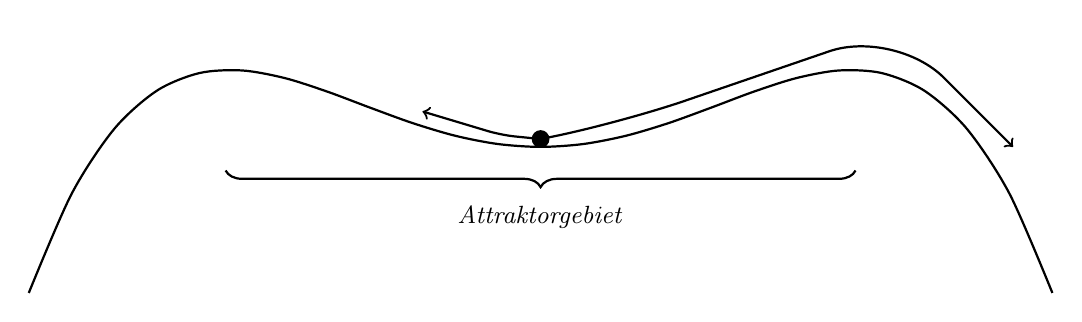
\begin{tikzpicture}

  % Curvy line
  \draw[thick, domain=-6.5:6.5, smooth, variable=\x] 
    plot ({\x}, {-0.004*(\x)^4+0.125*(\x)^2});
  % Ball 
  \filldraw[black] (0,0.1) circle (3pt);

  % Arrows
  \draw[->, thick, rounded corners=5pt] 
    (0,0.1) -- (-0.5,0.15) -- (-1.5, 0.45);
  \draw[->, thick, rounded corners=25pt] 
    (0,0.1) -- (1,0.3) -- (4.5,1.5) -- (6,0);

  % Label
  \draw[decorate,decoration={brace, mirror, amplitude=6pt}, thick] (-4,-0.3) -- (4,-0.3);
  \node at (0,-0.9) {\small \textit{Attraktorgebiet}};

\end{tikzpicture}
\end{center}

Den Bereich, in welchem Störungen kein Problem darstellen, das System also stabil bleibt, nennen wir Attraktorgebiet.
In der Praxis sind wir oftmals daran interessiert wie groß das Attraktorgebiet ist, also wie viel Störung verkraftbar 
ist, ohne dass unser System instabil wird.

Basierend auf dieser Idee wollen wir nun den Begriff der Pseudospektren im Kontext von Matrizen / Eigenwerten einführen.

Die Grundidee des Pseudospektrums kann jedoch auch in viel allgemeineren Situationen eingeführt werden. 
% Dunford \& Schwartz: Linear Operators
% Kato: https://doi.org/10.1007/978-3-642-66282-9


% Begriff der Pseudospektren geht auf Landau zurück. Viele Resultate von Trefethen etal. \\

% Das Konzept des Pseudospektrums ist bei normalen Operatoren die Vereinigung der 
% $\varepsilon$-Umgebungen seiner Eigenwerte 

\begin{colbox}{Definition}
  Für $\varepsilon\in\R_+$, ist das $\varepsilon$-Pseudospektrum $\sigma_\varepsilon(A)\subset\C  $ 
  einer Matrix $A\in\K^{n\times n}$ definiert als 
  \begin{align*}
    \sigma_\varepsilon(A) := \{z\in\C\backslash\sigma(A)\,:\, \vertn{2}{(A-zI)^{-1}}_2\geq \tfrac{1}{\varepsilon}\} 
    \cup \sigma(A)
  \end{align*}
\end{colbox}

\begin{colbox}{Bemerkung}
  Die Krylov-Unterraum-Methoden, die bisher diskutiert wurden, lassen sich zur Berechnung des Pseudo-Spektrums einer 
  Matrix verwenden. (z.B. bei der Matrix von diskretisierten partiellen Differentialgleichungen)
\end{colbox}

\begin{colbox}{Lemma}\label{lem:pseudoChar}
  \begin{enumerate}
    \item 
      Das $\varepsilon$-Pseudospektrum einer Matrix $T\in\C  ^{n\times n}$ kann definiert werden 
      durch
      %
      \begin{align*}
        \sigma_\varepsilon(T) 
        := \{z\in\C  \,|\,\sigma_{\min}(zI-T)\leq\varepsilon\}
      \end{align*}
      %
      wobei $\sigma_{\min}(B)$ den kleinsten Singulärwert der Matrix $B$ bezeichnet, d.h. 
      %
      \begin{align*}
        \sigma_{\min}(B) := \sqrt{\lambda_{\min}(B^HB)}
         % \min\{\lambda^{1/2}\,|\,\lambda\in\sigma(B^HB)\}
      \end{align*}
      %
    \item 
      Das $\varepsilon$-Pseudospektrum $\sigma_\varepsilon(T)$ einer Matrix $T\in\C  ^{n\times n}$ ist 
      invariant unter Orhtonormalen Transformationen, d.h. für eine unitäre Matrix $Q\in\C  ^{n\times n}$ 
      gilt $\sigma_\varepsilon(Q^*TQ) = \sigma_\varepsilon(T)$
  \end{enumerate}
\end{colbox}

\textit{Beweis.} 
\begin{enumerate}
  \item 
    Es gilt
    %
    \begin{align*}
      \vertn{2}{(zI-T)^{-1}}_2  
      &= \sqrt{\lambda_{\max}((zI-T)^{-H})(zI-T)^{-1}} \\
      &= \sigma_{\max}((zI-T)^{-1}) \\ 
      &= \sigma_{\min}((zI-T))^{-1} \\ 
    \end{align*}
    %
    Daraus folgt:
    %
    \begin{align*}
      \sigma_\varepsilon(T) 
      &= \left\{ z \in \C   \;\middle|\; \vertn{2}{(zI-T)^{-1}}_2 \geq \tfrac{1}{\varepsilon} \right\} \\
      &= \left\{ z \in \C   \;\middle|\; \sigma_{\min}(zI-T)^{-1} \geq \tfrac{1}{\varepsilon} \right\} \\
      &= \left\{ z \in \C   \;\middle|\; \sigma_{\min}(zI-T) \leq \varepsilon \right\}
    \end{align*}
    %
  \item \textcolor{red}{vgl. Aufgabe 10.1}
  \qed
\end{enumerate}

\textbf{Numerische Berechnung}\\
Zur näherungsweisen Bestimmung von $\varepsilon$-Pseudospektren einer Matrix $T$ betrachtet man in der Praxis eine 
diskrete Menge von Gitterpunkten $D\subset \C$ und berechnet alle Punkte $z_i\in D$ den kleinsten Singulärwert 
von $(z_i I - T)$. Diese Werte liefern nach Lemma \ref{lem:pseudoChar} das größtmögliche $\varepsilon$, so dass 
$z_i\in \sigma_{\varepsilon}(T)$. 

Anschaulich liefern die Pseudospektren eine Art Höhenprofilüber der komplexen Ebene, mittels Interpolation 
der Gitterwerte erhalten wir eine grafische Darstellung der zugehörigen Höhenlinien.
